\begin{figure}[ht]
\centering
\resizebox{\linewidth}{!}{
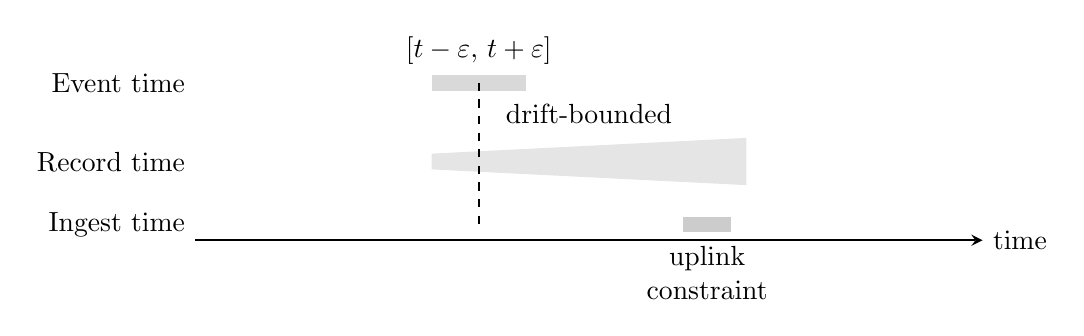
\begin{tikzpicture}[>=stealth, thick]

% Time axis
\draw[->] (0,0) -- (10,0) node[right] {time};

% Labels
\node[left] at (0,2) {Event time};
\node[left] at (0,1) {Record time};
\node[left] at (0,0.2) {Ingest time};

% Event time uncertainty band
\fill[gray!30] (3,1.9) rectangle (4.2,2.1);
\node[above] at (3.6,2.1) {$[t-\varepsilon,\, t+\varepsilon]$};

% Record time drift band
\fill[gray!20] (3,0.9) -- (3,1.1) -- (7,1.3) -- (7,0.7) -- cycle;
\node[above] at (5,1.35) {drift-bounded};

% Ingest time contraction
\fill[gray!40] (6.2,0.1) rectangle (6.8,0.3);
\node[below,align=center] at (6.5,0.05) {uplink\\constraint};

% Vertical projection
\draw[dashed] (3.6,2) -- (3.6,0.2);

\end{tikzpicture}
}
\caption{Temporal coherence with propagated uncertainty. Event time is represented as an interval whose uncertainty evolves across sensing, buffering, and uplink rather than collapsing into a single timestamp.}
\end{figure}
